SafeStreets is a distributed multilayer software application. The software architecture is a thin three-tiers architecture, based on the MVC design pattern:
\begin{itemize}
    \item \textit{Presentation layer (View)}: the presentation layer is conceived as an high level representation of the application, which will be responsible for the user and third party interaction and data visualization. Also, the presentation layer is the only gateway from which actors can interact with the system;
    \item \textit{Application layer (Controller)}: the application layer is responsible for the core functionalities of the system: inside the controller, the main functions and the business logic is embedded and performed whenever an actor requires their execution;
    \item \textit{Data layer (Model)}: the data layer is responsible for the interaction between the system and the data storage. It manages every operation performed by the system that requires data retrieving and storaging.
\end{itemize}
The logical separation (MVC) allows the system to preserve the safety of sensible data stored in the data layer, as users have only a restricted access to the presentation layer.
\begin{figure}[H]
    \centering
    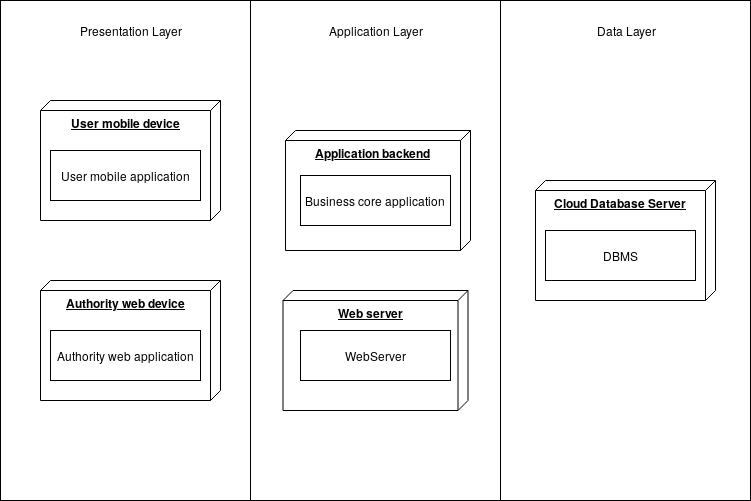
\includegraphics[width=1.0\textwidth]{UML_diagrams/overview_diagram}
    \caption{Overview diagram}
    \label{fig:overview_diagram}
\end{figure}
Analyzing the figure \ref{fig:overview_diagram} in details, it is possible to see how the layers are organized:
\begin{itemize}
    \item \textbf{Presentation layer}: the mobile application is run on the user mobile devices and distributed through the Android and IOS official stores. Moreover, the authority web application is accessible through any web browser at a specific URL.
    \item \textbf{Application layer}: a cluster of dedicated servers contains some replicated istances of the backend system that run accordingly to preserve a continuous functioning of the system. The application layer servers also have a local cache necessary for the computation of the ordinary system functionalities. Also, another cluster of servers contain the web server application on which the authority web app runs; 
    \item \textbf{Data layer}: data is stored on a cloud DBMS that guarantees a constant and consistent functioning. This allows to reduce the cost of maintainance of the system, as by paying a yearly subscription is much cheaper than running a cluster of server (cost of electricity and cooling systems) and performing periodic maintainance.
\end{itemize} 
%TODO: Inserisci grafico network
\begin{figure}[H]
    \centering
    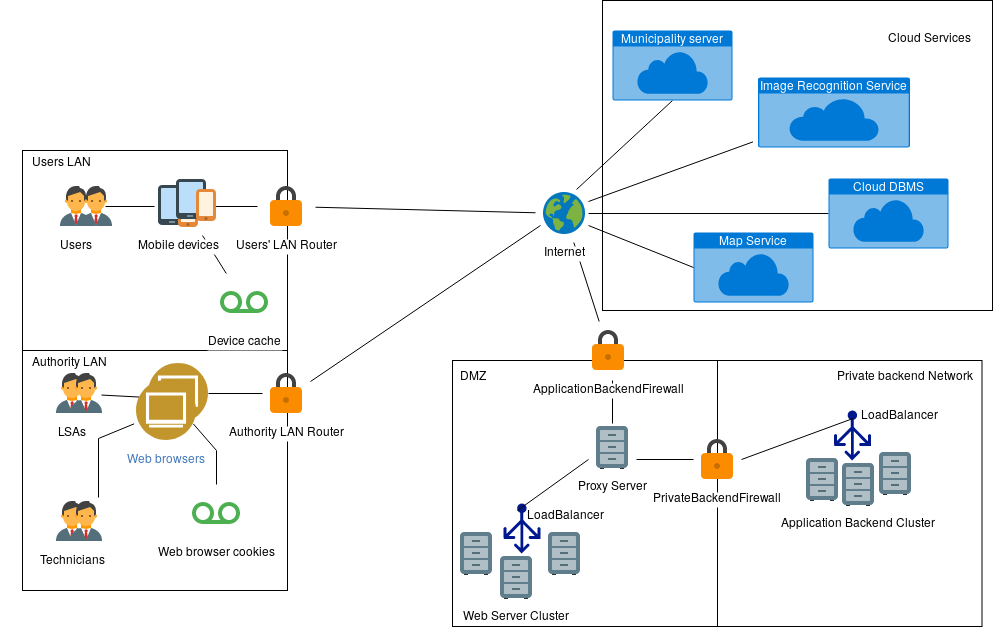
\includegraphics[width=1.0\textwidth]{UML_diagrams/network_diagram}
    \caption{Network architecture}
    \label{fig:network_diagram}
\end{figure}
The network architecture of the Safestreets system is described in the figure \ref{fig:network_diagram}. 
\begin{itemize}
    \item The presentation layer is phisically separated from the rest of the system by the LAN routers of users and authorities;
    \item The application layer is splitted in two main areas: 
        \begin{itemize}
            \item A DMZ (DeMilitarized Zone), in which a proxy server filters the requests coming from the internet and forwards them to the web server load balancer and to the private backend network;
            \item A private backend network, which has another router/firewall that filters once more the requests in order to guarantee an higher level of safety. Inside the private backend network, the system workflow is automatically balanced through a \textbf{load balancer} which forwards automatically the requests to the least stressed node in order to avoid bottlenecks and system overloading.
        \end{itemize}
    \item The data layer is represented as a cloud server (DBMS) and treated as a black box.
\end{itemize}
Also, the municipality server and the image recognition service have been pictured for completeness.\newline
This architecture allows the system to meet the non-functional requirements of flexibility and robustness already explained in the RASD document: 
the backend application is distributed on several nodes distributed on the same cluster, in order to guarantee a corrected and continuous functioning. In case a node crashes, another one is able to take its place automatically and keep the system running. For this purpose, it is necessary to highlight the fact that all nodes are consistent copies of each others: data and logic functions are kept consistent through automatic techniques of node replication that preserves the ACID rules.  
\newline As it is possible to evince in the figure \ref{fig:network_diagram}, the web servers, backend and data nodes are replicated independently and separately.
The division is necessary in order to isolate and preserve the system core functions. This practice is made for:
\begin{itemize}
    \item \textit{Safety purposes}: having phisically separated nodes prevent the possibility to reach certain hidden layer (for example the data layer) of the system, which needs to be absolutely safe as they contain sensible data.
    \item \textit{Maintainance purposes}: when maintainance is performed over a certain part of the system, this separation allows to preserve that part of the system which does not require maintainance;
    \item \textit{Node migration}: if the system will require to be partially moved from a cluster to another in the future, this division allows to transfer only a specific part of the network without the need of transferring the whole system.
\end{itemize}


%TODO: aggiungere acronimo di URL
